\documentclass[a4paper, 12pt, oneside]{book}

%% packages
\usepackage[backend=biber,style=ieee]{biblatex}
\usepackage{graphicx} % for including images
\usepackage{hyperref} % for clickable embeded links (including in-doc refs)
\usepackage{minted} % for code highlighting
\usepackage{nameref} % for in-doc references | \labal{} |  \ref{}  \nameref{}
\usepackage{booktabs} % for midule
\usepackage{siunitx} % for midrule
\usepackage{amsmath,amssymb} % for expectation sign
\DeclareMathOperator{\E}{\mathbb{E}}
\usepackage[vlined, ruled]{algorithm2e}
\usepackage[table]{xcolor}
\usepackage{multirow}
\usepackage{luatexja-fontspec}

\newcolumntype{L}[1]{>{\raggedright\let\newline\\\arraybackslash\hspace{0pt}}m{#1}}
\newcolumntype{C}[1]{>{\centering\let\newline\\\arraybackslash\hspace{0pt}}m{#1}}
\newcolumntype{R}[1]{>{\raggedleft\let\newline\\\arraybackslash\hspace{0pt}}m{#1}}

%% chapter starting from 1
\setcounter{chapter}{0}

%% bibliography
\addbibresource{./src/bibliography.bib}

\begin{document}

%% use roman page numbering for abstract and acknowledgements
\pagenumbering{roman}

%% title page
\begin{titlepage}
\begin{center}
    \vspace{0.1\textheight}
    {\Large Undergraduate Thesis 2022} \\
    \vspace{0.05\textheight}
    
\includegraphics[width=48truemm]{resources/0_title/waseda_logo.png} \\
    \vspace{0.05\textheight}
    \textbf{\huge Campus as 'Canvas': Regional Revitalization in general with location-based Augmented Reality and Co-creation} \\
    \vfill
    {\Large Supervisor \hspace{0.02\textwidth} Nakajima Tatsuo} \\
    {\Large Area of Study \hspace{0.02\textwidth} Computer Science} \\
    \vspace{0.05\textheight}
    {\Large 
        Waseda University \\
        School of Fundamental Science and Engineering \\
        Department of Computer Science \\}
    \vspace{0.05\textheight}
    {\Large 1W17BG08-2 Hu Yong-Hao \\}
    \vspace{0.05\textheight}
    {submitted on 2022.01.31}
\end{center}
\end{titlepage}

%% abstract
\pagebreak
\hspace{0pt}
\vfill % magic commands to vertically center the content
    \begin{center}
    Abstract
    \end{center}
Pandemic and digitalization results in an increase of places or facilities becoming desolate or abandoned.
Since both location-based AR and co-creation have been proved to have influence on users' motivation and the places they are implemented,
for revitalization of places in general, we composed a framework consisting of location-based AR and co-creation together.
We developed a prototype with components described in the framework, and then we conducted an experiment where participants used the prototype in Nishi-Waseda campus of Waseda University.
Results showed positive influence of location-based AR and co-creation on participants' motivation to access the campus and images of the campus in their mind,
which indicated the feasibility for our framework to revitalize the campus. We then discussed its generalization to other public facilities.
Limitations in this study include restrictions in AR experience and ambiguous evaluation for certain items, and we also suggested future directions to improve the limitations as well as further evaluate the generalization of the proposed framework.
\vfill
\pagebreak

%% acknowledgement
% \pagebreak
% \hspace{0pt}
% \vfill 
%     \begin{center}
%     Acknowledgements
%     \end{center}
% This is my acknowledgements...

% \vfill
% \pagebreak

%% use normal page numbering for the main body
\pagenumbering{arabic}

%% table of contents 
\tableofcontents
\listoffigures 
\listoftables

%% main body
\clearpage
% % \chapter{Notations}
% Sample notations \autoref{ta:notations}

% % table of notation
% \setlength{\tabcolsep}{6pt}
% \begin{table} 
% \begin{center} 
% \caption{Mathematical notations}
% \label{ta:notations}
% {\normalsize
% \begin{tabular}{l c}
% \toprule
% Symbol & Meaning \\
% \midrule
%     $\alpha$ & learning rate\\
%     $\gamma$ & discount factor \\
%     $S, s$ &   state \\
%     $A, a$ &   action \\
%     $R, r$ &   reward \\
%     $\tau$ &    a trajectory / an episode \\
%     $G$ &   return \\
%     $t$ &   a discrete time step \\
%     $G_t$ & return at time step t \\
%     $T$ &   final time step of an episode \\
%     $\pi$     & policy \\
%     $\pi_\theta$ & parametrized policy with parameter \theta \\
%     $\pi(s)$ & the action distribution given state $s$ under policy $\pi$ \\
%     $\pi(a|s)$ & probability of action $a$ given state $s$ under policy $\pi$ \\
%     $\E$ & expectation \\
%     $\E_\pi$ & expectation under policy $\pi$ \\
%     $v(s)$ & state value of state $S$ \\
%     $v_\pi(s)$ & state value of state $S$ under policy $\pi$\\
%     $q(s, a)$ & action value of action $a$ on state $s$ \\
%     $q_pi(s, a)$ & action value of action $a$ on state $s$ under policy $\pi$\\
%     $\sigma$ & activation function \\
% \bottomrule
% \end{tabular}
% } \end{center} \end{table}
% \setlength{\tabcolsep}{6pt}





\chapter{Introduction}
% Topic

\section{Motivations}
% Current situations
% Why there needs further research

As the pandemic of COVID-19 spreading throughout the world since 2020,
people were forced or encouraged to stay home and restricted from accessing public places,
including tourist attractions, shops, workplaces, schools, etc.
Humans' freedom in physical space is restricted, which accelerate the progress of digitalization.
Not only entertainment but more and more economic and even academic activities are moving online.
As the pandemic slowing down recently, despite the resumption of some physical activities,
there are places or facilities remaining unused or abandoned due to financial problems,
amount of users not recovered, digitalization of activities, and so on.

Removing the idle places or facilities is a choice, but if it is possible to give them new values or change people's image of them,
they can play different roles and keep contributing the society or enrich the environment.
In fact, the concept 'Regional Revitalization', which referes to the attempts to vitalize rural towns where population is falling,
by making use of local speciality combined with new ideas to develop new and unique industries such as tourism, has been applied around Japan recently.
Among cases of Regional Revitalization, some of them adopt location-based Augmented Reality to help enrich the space.
Location-based Augmented Reality is defined as Augmented Reality that utilize geographical information to display contents corresponding to a physical location.
It has already used in not merely entertainment, where Pokemon GO is a famous example,
but also implemented in tourism and education, which implies its versatility and practicability.
With the application of location-based Augmented Reality and the reference of Regional Revitalization,
transformation of an idle place or facility without physical reconstruction seems to be feasible.

% BUT not all places are tourist attractions; each place has its unique features and original functionalities; customizing contents for each place is difficult
  % -> Common characteristics: People!
  % -> Enable people to create new values / images for the place (co-creation)
% BUT how to encourage people?
  % -> User-user interaction!

\section{Objectives and importance}
% RQ
【RQ】Location-based AR+ユーザ共創のコンテンツが:
ある場所をもっと魅力的にする?
ある場所がユーザにとっての意義が変わる?
ユーザ同士の交流ができている?

% goals
キャンパスの元気を取り戻す and answer the RQs
propose a general model to vitalize an arbitrary place

% hypotheses
significant, positive effect

% importance
* (Preliminary studies of) Local transformation in general, instead of only tourism or education goals
* Use ‘people’ to comprise the contents, instead of considering specific characteristics of each location
* Prove a possibility, instead of focusing on detailed improvement of technology
    * Future work: combined with improved technology

\section{Overview of this paper}
% order of sections in this paper
% outline the methodology

\section{Sample section}

Sample template \cite{alphago}

\begin{figure}
  \centering
  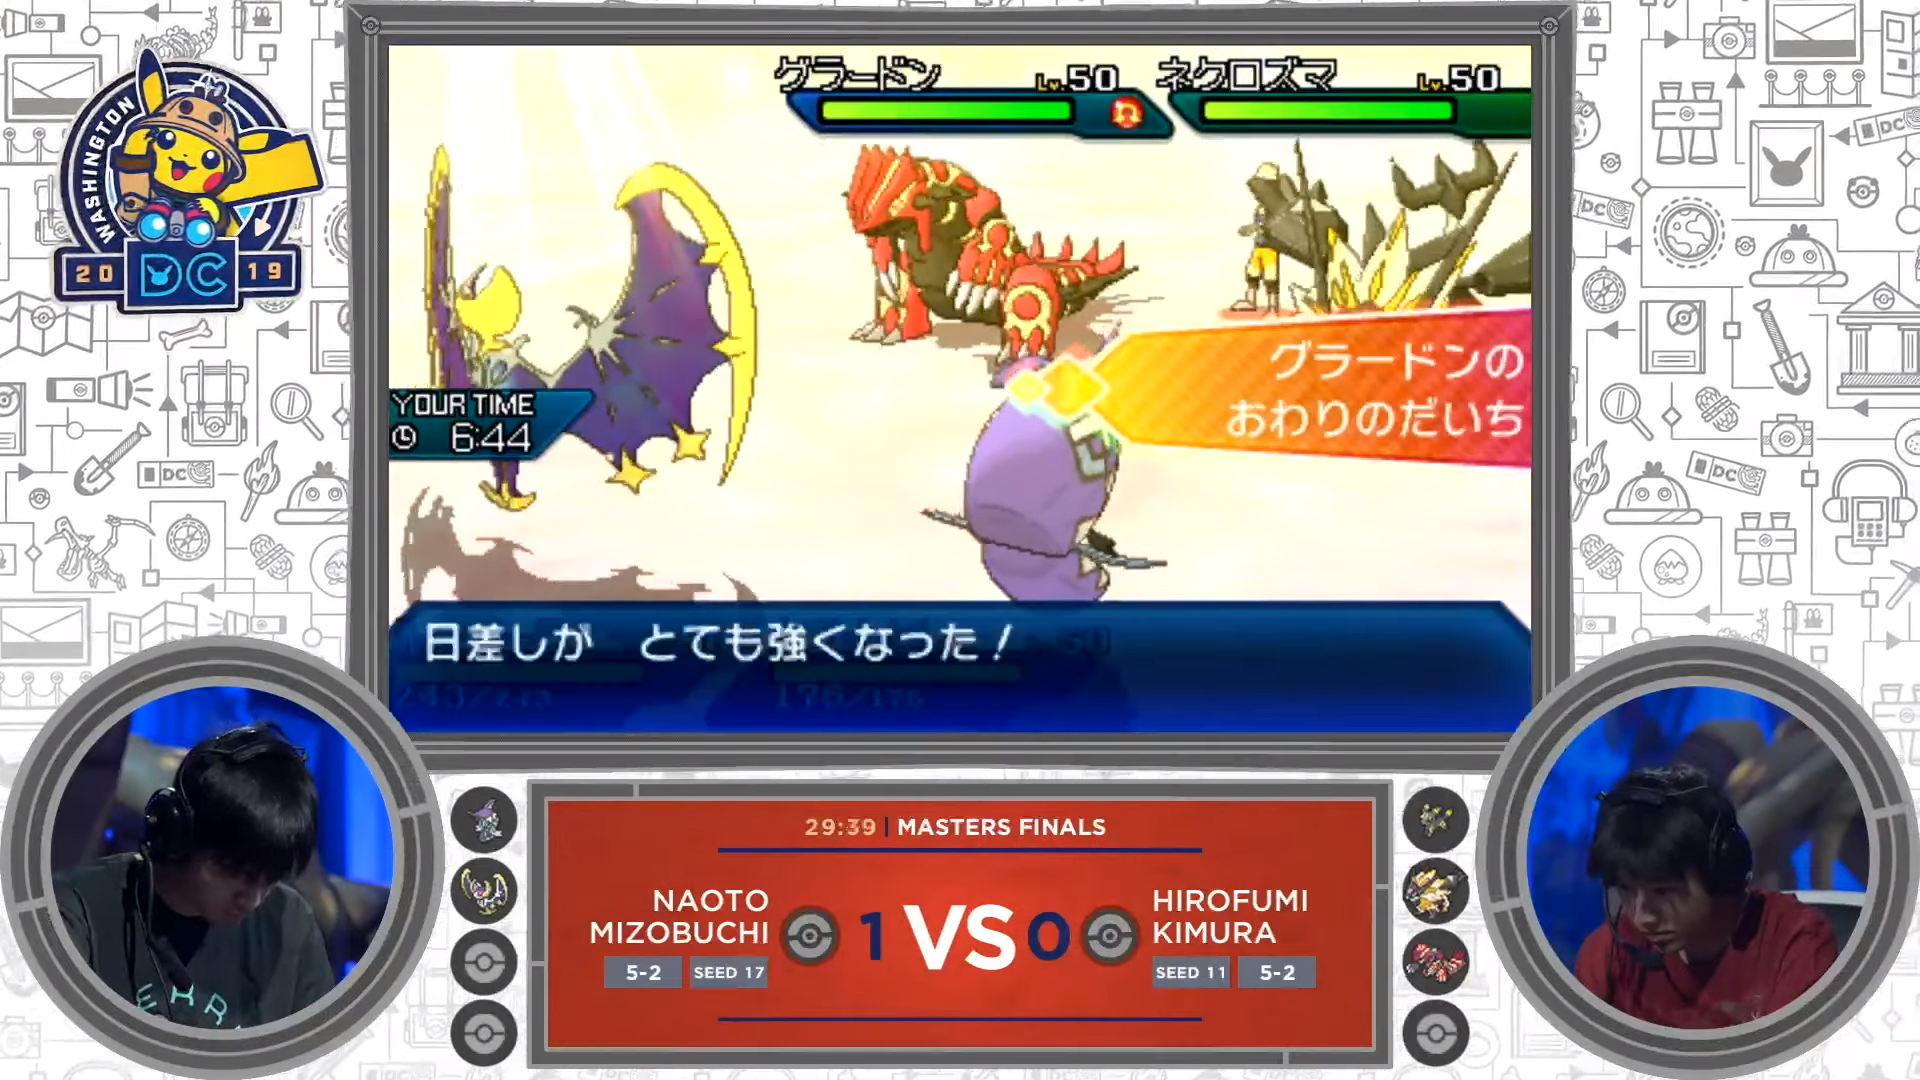
\includegraphics[width=\columnwidth]{resources/1_intro/vgc2019.png}
    \caption{Screenshot of the Grand Finals of the Pokemon Video Game Championships 2019 held in Washinton D.C.}
\end{figure}


\chapter{Backgrounds} \label{ch:2}
% Explain concepts required to understand this paper, with including references to existing works that introduced the concepts

\section{Pandemic's impact}

Google has been collecting their users' mobility data since the beginning of 2020 \cite{googlemobilityreports} \cite{ourworldindata_2020}.
Results indicate that people do access public places, including transit stations, workplaces and parks, less than before pandemic started spreading.
The pandemic also accelerate the process of digitalization \cite{amankwah-amoah_khan_wood_knight_2021}, which also resulted in a decrease of people commute physically.
There are also investigations indicating that more than tens of thousands of store closed in Japan during the pandemic.
Other investigations show that remote working has becoming a permanent phenomenon around the world \cite{saad_wigert_2021}.
In Japan, government even made a policy to discourage employees to commute physically.
The above situations resulted in more unused facilities left on the society.
The U.S. government holds about 45,000 underused or underutilized buildings according to an investigation by Harvard Business Review \cite{hounsell_2020}.

\section{Local Revitalization}
Local Revitalization is proposed by Japanese government, aiming at combining local unique features or specialties and new ideas or technology,
in order to stimulate rural economics to balance the gap between cities and rural areas \cite{sawaji_2019}.

Common approaches include improving quality or design of existing local products with new techniques, launching new industries with local features, and broadening promotion on SNS or other media.
Of course, a standard does not exist in the field of Local Revitalization, and there are different cases adopting diverse approaches,
such as inserting real landscapes or local products into dramas or animations to attract audience,
or inviting artists to create graffiti at shopping streets to get their customers back \cite{中野経済新聞_2015}\cite{サンテレビニュース_2021}\cite{urbact_2019}.

As the development of Augmented Reality, there are also cases implementing Augmented Reality in their revitalization projects,
such as placing a virtual castle on a historical ruin \cite{井上道哉_長澤可也_2021} and displaying interactive digital contents beside local physical exhibits \cite{センチメンタル価値再生_2016}\cite{armarker_and_behavior_log_2011}.

\section{Location-based Augmented Reality}
Augmented Reality (AR) utilizes camera on smartphone or glasses to capture the landscape of real world,
and then displays digital contents on the captured landscape so as to combine digital information with reality.
Location-based Augemnted Reality makes use of geographical information such as GPS data or feature points of a landscape,
so that displayed contents are located corresponding to a specific location.
Pokémon Go is one of the famous cases of Location-based AR, which displays virtual characters 'pokemons' based on geographic coordinates around the world and requires players to move physically to catch them \cite{pokemongo_homepage}.
The game has earned more than 5 billion dollars since its launch 5 years ago \cite{strategist_2021}, indicating the enormous popularity it possesses.

Beside entertainment, Location-based AR is also applied in tourism and education cases,
including displaying educational resources on a tablet when getting close to a spot in an archaeological site \cite{law_2018},
or asking a user to challenge a quiz on one's smartphone when approaching a historical building \cite{hwang_chang_chen_chen_2017}.

\section{Co-creation}
Co-creation, in business context, is defined as a company involving its customers in the creation of products or services to suit customers' own context \cite{cocreation_definition}.
In a general context, it is also defined as any act of creativity that is shared by two or more people \cite{cocreation_definition_general}.
Co-creation can happen not merely between a company and its customers but also in occasions where value creation is conducted by ordinary people together \cite{cocreation_general_case}.
% examples in other fields (check yilmaz_2021)

In our study, we adopt the more general definition, and we also refer to researches about co-creation in business or other context,
which will be introduced in the next chapter.
\chapter{Related Works} \label{ch:3}
% summarize existing related / similar works, and discuss how my paper differs from them

\section{Location-based AR's effect on a place / how users view the place}
Hwang et al. developed a location-based AR learning system for supporting local culture courses.
For students who used the system in field trips, an enhancement in their local culture identity,
identification of the culture in a place where one lives, is observed \cite{hwang_chang_chen_chen_2017}.
Law created a mobile app which features a navigation map and pop-ups of educational resources when a user approaches a site physically,
and the study implicates the potential of location-based AR to enhance and disseminate the value of cultural heritage \cite{law_2018}.
These studies investigate the influence of Location-based AR on the place or on how people value the place,
while they focus more on educational goals, and their systems were developed for specific cases, which requires more knowledge and cost to implement.

Chan et al. attempted to integrate location-based AR and virtual currency to connect travelers and local shops,
form a new tourism ecosystem and further build an offline business network \cite{chan_lin_wang_lu_hsu_2017}.
The system Chan et al. developed is less case-specific, but their investigation is only adapted to the field of tourism business.

Therefore, we began to be curious about the influence of Location-based AR on the place or on how people value with a more general and less case-specific investigation.

\section{Location-based AR's effect on users' motivation}
Laato et al. found that a location-based AR game motivates players to go outside even during pandemic \cite{laato_islam_laine_2020}.
Lee et al. proposed a framework describing reasons of stickness to location-based AR game,
and their analysis indicates positive influences by satisfaction and sense of flow \cite{lee_chiang_hsiao_2018}.
Both of the studies chose Pokemon GO as their target to analyze how Location-based AR affects users' motivation,
while Pokemon Go's gaming features are also included in their proposed model.
Despite Pokemon GO's leading awareness among all location-based AR games,
Lee et al. pointed out that other location-based AR games also deserve investigation \cite{lee_chiang_hsiao_2018},
and we consider that an examination on not a game but a more general location-based AR service would be more representative.

Lacka's assessment indicates that full-fledged location-based AR games played in tourism destination support users to acquire knowledge about the place,
which subsequently enhances users' visit intention \cite{lacka_2018}.
Research conducted by Chan et al. mentioned above also investigated how their AR implementation motivates travelers to engage in more extensive and deeper travel experiences \cite{chan_lin_wang_lu_hsu_2017}.
Lacka focused more on tourism and learning aspects, and Chan et al. also investigated about tourism, which are the most focused fields in researches about AR recently,
and we believe that more investigations of motivation from other aspects would help location-based AR be applied in more situations.

\section{Co-creation's effect on a place and users' motivation}
Destination image, a term in tourism context, is defined as the aggregation of people's subjective perception,
including beliefs, ideas and impressions, associated with a destination \cite{kotler_haider_rein_2008}\cite{Lopes2011DestinationIO}.
Yilmaz's paper points out the lack of studies about how destination image occurs over time, despite destination image being studied much in tourism literature,
and the paper presents an approach to realize the formation of destination image with co-creation \cite{yilmaz_2021}.
Vries et al. built a model of antecedents of destination image co-creation and examine the effect of each antecedent \cite{glyptou_2021}.

The concept of destination image is similar with our idea about people's image of a location,
and both Vries et al. and Yilmaz's researches about destination image with co-creation indicate the potential of co-creation to influence people's image of a location in our study.

In addition, Vries et al. examined about customer engagement with Facebook brand pages, and they confirmed the influence of co-creation value on customer engagement \cite{vries_carlson_2014},
which we consider as a precedent to prove co-creation's possibility to improve users' motivation.

The studies introduced above focus specifically on tourism or business viewpoint, which provides us a room to develop our study in a broader context.

\section{User-user interaction's effect on engagement with co-creation}
Studies show that desire to contact or socializing between users motivate users to participate in co-creation activities \cite{fernandes_remelhe_2016}\cite{engstrom_elg_2015}.
Waseem et al. also found that interpersonal engagement is one of the key drivers that evoke motivations among employees to facilitate value co-creation \cite{waseem_biggemann_garry_2020}.
The influence of community in triggering users to engage in co-creation is examined as well \cite{palma_trimi_hong_2018}\cite{zhang_kandampully_bilgihan_2015}.
From these studies we confirmed that interaction between users works well on motivating people to participate in co-creation,
so we attempted to include interaction between users into our work as well to examine its effect on the context of co-creation with location-based AR.

\section{Location-based service or AR with Co-creation}
Cases of co-creation implemented in location-based services or AR application also emerged in recent years.
Anttoni Lehto et al. presented an adoption of co-creation which allowed students to initially create contents for a location-based AR learning platform \cite{lehto_lautkankare_brander_alanissila_saari_salminen_2020}.
Jorge Bacca et al. proposed a framework to utilize co-creation in designing motivational augmented reality for vocational education and training \cite{acosta_navarro_gesa_kinshuk_2019}.
Alavesa et al. developed a location-based AR client for their living labs, which is described as an environment involving users into innovation \cite{alavesa_2018}.
Leung et al. proposed a smart service network to realize co-creation of interactive dining experiences using location information \cite{leung_loo_2020}.
Slingerland et al. include users in the design of game activities to examine what kind of location-based activities citizens prefer to interact with neighbours and explore their neighbourhood \cite{slingerland_fonseca_lukosch_brazier_2020}.
With such a number of precedents, we believe that our idea, which includes implementation of location-based AR and co-creation together, is worth to be conducted and examined.

% add figures from the VC paper
\chapter{Methodology}\label{ch:4}

\section{Proposed Framework}
Reviewing a variety of regional revitalization cases, we sketched a diagram at Figure 4.1 to summarize their common mechanism.
In a common case of regional revitalization, the authority makes use of local specialties and applies new ideas with technology to improve existing industry or establish a new one,
usually a tourism business, which succeeds to attract more people to visit the place and activate local economy.

We also sketched a diagram at Figure 4.2 to describe a common mechanism of regional revitalization that implements location-based AR.
In such cases, the authority applies new ideas on local features to compose unique contents for a location-based AR service,
which motivates people to access the place more, resulting in an improvement in local economy.
Despite that the contents are in digital form or accessible online, the system's location-based characteristics still make it to encourage visitors to access physically.

\begin{figure}
  \begin{minipage}{0.48\textwidth}
    \centering
    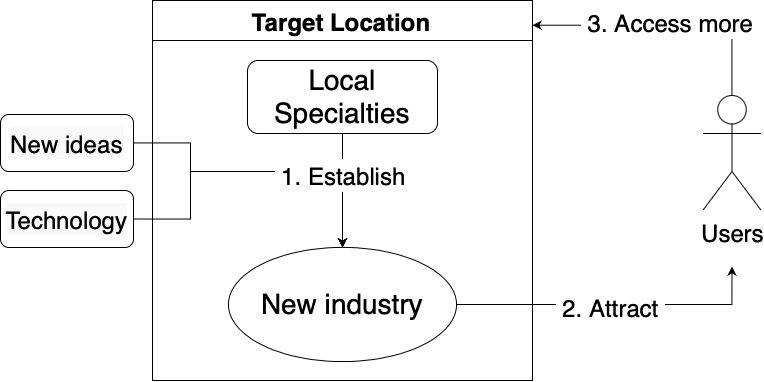
\includegraphics[width=0.9\linewidth]{resources/4_methodology/common_vitalization.png}
      \caption{Common framework of Regional Revitalization}
  \end{minipage}\hfill
  \begin{minipage}{0.48\textwidth}
    \centering
    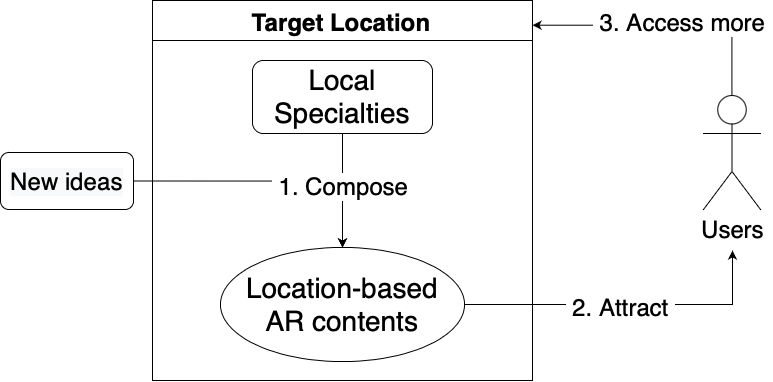
\includegraphics[width=0.9\linewidth]{resources/4_methodology/revitalization_with_AR.png}
      \caption{Framework of Regional Revitalization with location-based AR}
  \end{minipage}
\end{figure}

For places like public facilities where there is a lack of local features usable to attract visitors,
we presented a framework, sketched in Figure 4.3, that adopts a common characteristic of the places: users.
In our assumption, by enabling users to engage in co-creation of contents, which can be conducted digitally with low costs in a location-based AR system,
we anticipate that the problem of lacking usable resources becomes solvable.
Besides the issue of content creation, From Section 3.1, 3.2 and 3.3 we understand the influence on users' motivation and images about a place by both location-based AR and co-creation,
which are both included in our framework.
We also introduce a socializing mechanism to encourage users to participate in the co-creation process.
From Section 3.4 we understand that interaction between users improves people's engagement with a co-creation activity.

For this framework we proposed, we developed a prototype according to the idea of the framework, and later we examined the proposed framework with an experiment with the prototype.

\begin{figure}
  \centering
  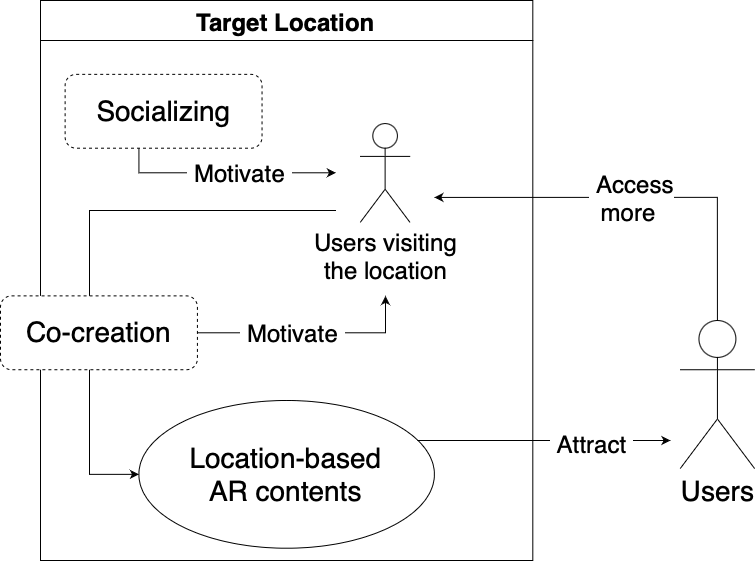
\includegraphics[width=0.8\columnwidth]{resources/4_methodology/revitalization_with_AR_and_cocreation.png}
    \caption{Proposed framework: Revitalization with location-based AR and Co-creation}
\end{figure}


\section{Prototype}

\chapter{Experiment and Results}\label{ch:5}

\section{Questionnaires}

\section{Experiment}

\section{Results}
\subsection{Motivations}

\subsection{Image of Campus}

\subsection{User-user Interaction}
\chapter{Results and Discussion}\label{ch:6}

\section{Motivations}

\section{Image of Campus}

\section{User-user Interaction}

\chapter{Conclusion}\label{ch:7}

In this study, we proposed a framework consisting of location-based AR, Co-creation and user-user interaction for revitalizing a general place.
We expected that the combination of location-based AR and Co-creation makes a place more attractive and brings it new images, and we also expect user-user interaction motivates people to access the place.
We developed a prototype following the framework and conducted an experiment with participants using the prototype in Nishi-Waseda campus, and the results evaluated by scales and free responses matched our expectation,
indicating that our framework is feasible for revitalization of the campus.
We then discussed its generalization to other public facilities.

Limitations of this study include the technological restriction related to location-based AR, lack of objective evaluation scales for changes in image of the place,
ambiguous evaluation results due to unclear definition of user-user interaction mechanism during the evaluation, and the concern for weather and pandemic.

The prototype in our study only allows 2D graffiti with mobile devices, although we made it to display the graffiti in different angles.
For future works adopting our proposed framework, to improve user experience, we suggest implementing a 3D sketching system like the one developed by Arora et al. \cite{arora_habib_kazi_grossman_fitzmaurice_singh_2018}, but the equipment issues should be solved first to make it usable outside the lab.
Improvement in GPS accuracy for mobile devices may also help improve the user experience.

For evaluation in future works, we suggest conducting control experiments with regard to different components in the framework to clarify their relevance between each other.
We also suggest designing a new scale for evaluating changes in the image of a general place, instead of the scale for destination image which is limited to tourism context, for more objective results.
Eventually, experiments in more diverse places are recommended in order to further evaluate the feasibility of generalizing our framework.

%% bib
\printbibliography

%% appendix
\appendix
\chapter*{APPENDIX A - Questions adopted from SIMS}

\begin{table}[h]
\begin{center}
\caption{Questions adopted from SIMS}\label{table:8}
\begin{tabular}{C{2cm} | l | C{1.9cm}}
    \hline
    \rowcolor{lightgray}
        \multicolumn{1}{C{2cm}}{Motivation \newline type} & \multicolumn{1}{c}{Questions} & \multicolumn{1}{C{1.9cm}}{Scale} \\
    \hline
    \multirow{4}{2cm}{Intrinsic motivation (IM)} & Because I think it is interesting. & \multirow{4}{1.9cm}{1 Disagree - 6 Agree} \\
        & Because I think it is pleasant. & \\
        & Because this is fun. & \\
        & Because I feel good when experiencing it. & \\
    \hline
    \multirow{4}{2cm}{Amotivation (AM)} & Personally I don't see any good reason to do it. & \multirow{4}{1.9cm}{1 Disagree - 6 Agree} \\
        & I'm not sure if it is worth it. & \\
        & I don't see what it brings me. & \\
        & I'm not sure it is a good thing to do. & \\
    \hline
\end{tabular}
\end{center} 
\end{table}


\chapter*{APPENDIX B - Free responses of changes in image of the campus}

\begin{table}[h]
\begin{center}
    \caption{Free responses of changes in image of the campus by viewing location-based AR contents}\label{table:9}
    \begin{tabular}{L{\textwidth}}
        \hline
        \rowcolor{lightgray}
          \multicolumn{1}{c}{Free responses} \\
        \hline
          {
            \begin{itemize}
              \item When I think other people draw at the place in campus, I want to check their artworks.
              \item I started to see places which I don't normally see.
              \item Many of the graffiti made things on campus look like something else, so the next time I saw it, I could think of the graffiti.
              \item I hadn't had a chance to take a good look at the campus, so it was refreshing.
              \item I couldn't draw pictures well, so I felt that there was a lack of reality (a sense of match with the real world).
              \item I tended to feel like I'm the only one in the campus, but when I think that everyone came to the university and looked at this remote place through the app, it brings something to my heart. It makes me feel closer to them.
              \item I used to feel that the campus was quiet and there was little interaction between people, but through this content, I learned that I could interact with strangers, and my image of the campus became more sociable.
              \item The campus became a little more fun, but it wouldn't have changed my overall image.
              \item To me it was just an application on phone where I can draw and see others' works
            \end{itemize}
          } \\
        \hline
    \end{tabular}
\end{center} 
\end{table}

\begin{table}[h]
    \begin{center}
      \caption{Free responses of changes in image of the campus by participation in co-creation}\label{table:10}
      \begin{tabular}{L{\textwidth}}
        \hline
        \rowcolor{lightgray}
          \multicolumn{1}{c}{Free responses} \\
        \hline
          {
            \begin{itemize}
              \item I began to look for a place where I could paint.
              \item I started looking at places I don't normally look.
              \item I started to think sometimes about what things on campus could look like.
              \item It's like we're all looking at the same place.
              \item I felt as if even the scenery I usually see is art from certain angles.
              \item I used to have an image of the campus as "less social", but this content has changed my image to "more sociable".
            \end{itemize}
          } \\
        \hline
    \end{tabular}
\end{center} 
\end{table}

\begin{table}[h]
    \begin{center}
      \caption{Free responses of changes in image of the campus by interaction between users}\label{table:11}
      \begin{tabular}{L{\textwidth}}
        \hline
        \rowcolor{lightgray}
          \multicolumn{1}{c}{Free responses} \\
        \hline
          {
            \begin{itemize}
              \item I went to more places when there were other users.
              \item We started to talk about the building and other things.
              \item I thought that since the interaction was with people, it had little impact on the image of the campus.
              \item I developed a common feeling that we were all students at the same university.
              \item There were pictures that made me wonder if that was the way to think.
            \end{itemize}
          } \\
        \hline
    \end{tabular}
\end{center} 
\end{table}

\begin{table}[h]
    \begin{center}
      \caption{Free responses of changes in image of the campus by overall experience}\label{table:12}
      \begin{tabular}{L{\textwidth}}
        \hline
        \rowcolor{lightgray}
          \multicolumn{1}{c}{Free responses} \\
        \hline
          {
            \begin{itemize}
              \item Overall, I started to pay more attention to the campus.
              \item I started to look at things on campus as different things, and remembered that other people had looked at things like this
              \item The campus had a gloomy image, but it changed to a sociable one.
            \end{itemize}
          } \\
        \hline
    \end{tabular}
\end{center} 
\end{table}

\chapter*{APPENDIX C - Free responses of preference between prototype at campus or situation at home}

\begin{table}[h]
  \begin{center}
    \caption{Example responses of preference between prototype at campus or situation at home by viewing location-based AR contents}\label{table:13}
    \begin{tabular}{C{2.5cm} | L{10cm}}
      \hline
      \rowcolor{lightgray}
      \multicolumn{1}{C{2.5cm}}{Preference} & \multicolumn{1}{c}{Example responses} \\
      \hline
        At campus & {
          \begin{itemize}
            \item It's easier for your brain to connect the actual place with the place in the graffiti.
            \item It gives a strong sense of actual experience and interaction.
            \item ... sitting at home and watching graffiti with pictures of the campus in the background makes it obvious that you are outside of that world. I believe that the experience you get will be completely different.
          \end{itemize}
        } \\
        \hline
        At home & {
          \begin{itemize}
            \item I couldn't help but notice the eyes around me.
            \item It's exhausting to travel around to check out the graffiti.
            \item I am more an indoor type person
          \end{itemize}
        } \\
      \hline
  \end{tabular}
\end{center} 
\end{table}

\begin{table}[h]
  \begin{center}
    \caption{Example responses of preference between prototype at campus or situation at home by participation in co-creation}\label{table:14}
    \begin{tabular}{C{2.5cm} | L{10cm}}
      \hline
      \rowcolor{lightgray}
      \multicolumn{1}{C{2.5cm}}{Preference} & \multicolumn{1}{c}{Example responses} \\
      \hline
        At campus & {
          \begin{itemize}
            \item It is more fun to draw on the spot.
            \item In the case of drawing at home, I didn't have as much freedom to choose my point of view as I did on campus, so it would be more interesting to draw on campus to explore different perspectives.
            \item I feel that it is important to draw while actually seeing buildings and other structures.
          \end{itemize}
        } \\
        \hline
        At home & {
          \begin{itemize}
            \item I can draw more calmly at home.
            \item I can paint without worrying about passersby.
          \end{itemize}
        } \\
      \hline
  \end{tabular}
\end{center} 
\end{table}

\begin{table}[h]
  \begin{center}
    \caption{Example responses of preference between prototype at campus or situation at home by interaction between users}\label{table:15}
    \begin{tabular}{C{2.5cm} | L{10cm}}
      \hline
      \rowcolor{lightgray}
      \multicolumn{1}{C{2.5cm}}{Preference} & \multicolumn{1}{c}{Example responses} \\
      \hline
        At campus & {
          \begin{itemize}
            \item I felt like we should be interacting in a real place.
            \item I would still prefer the real world interaction with other users at campus since it's easier to understand people's feelings and have a conversation.
            \item If you don't experience it at the place, you won't feel the realism and it won't be as interesting.
          \end{itemize}
        } \\
        \hline
        At home & {
          \begin{itemize}
            \item I thought that if the main purpose is to interact with people, there is no need to be on a campus.
            \item I felt that if we were just going to doodle together, we could do it online, like an online drawing chat, because it's easy to do at the same time.
          \end{itemize}
        } \\
      \hline
  \end{tabular}
\end{center} 
\end{table}

\begin{table}[h]
  \begin{center}
    \caption{Example responses of preference between prototype at campus or situation at home by overall experience}\label{table:16}
    \begin{tabular}{C{2.5cm} | L{10cm}}
      \hline
      \rowcolor{lightgray}
      \multicolumn{1}{C{2.5cm}}{Preference} & \multicolumn{1}{c}{Example responses} \\
      \hline
        At campus & {
          \begin{itemize}
            \item I could do it face-to-face with other users, and I could only encounter the artwork when I went there.
            \item ... using at campus is more interesting because you can choose your point of view more freely.
            \item If you don't experience it at the place, you won't get the sense of realism and it won't be as interesting. If you are there, you will be able to observe the actual situation more closely, which will give you more ideas for your doodles.
          \end{itemize}
        } \\
        \hline
        At home & {
          \begin{itemize}
            \item I can doodle without worrying about what others passed by.
            \item It's hard to concentrate when using it outside by yourself due to various factors such as temperature and people passed by.
          \end{itemize}
        } \\
      \hline
  \end{tabular}
\end{center} 
\end{table}


\addcontentsline{toc}{chapter}{APPENDIX A}  % unnumbered chapters are not added to TOC by default so adding it automatically



\end{document}

